\begin{figure}[!ht]
    \begin{minipage}{0.65\textwidth}
        \centering
        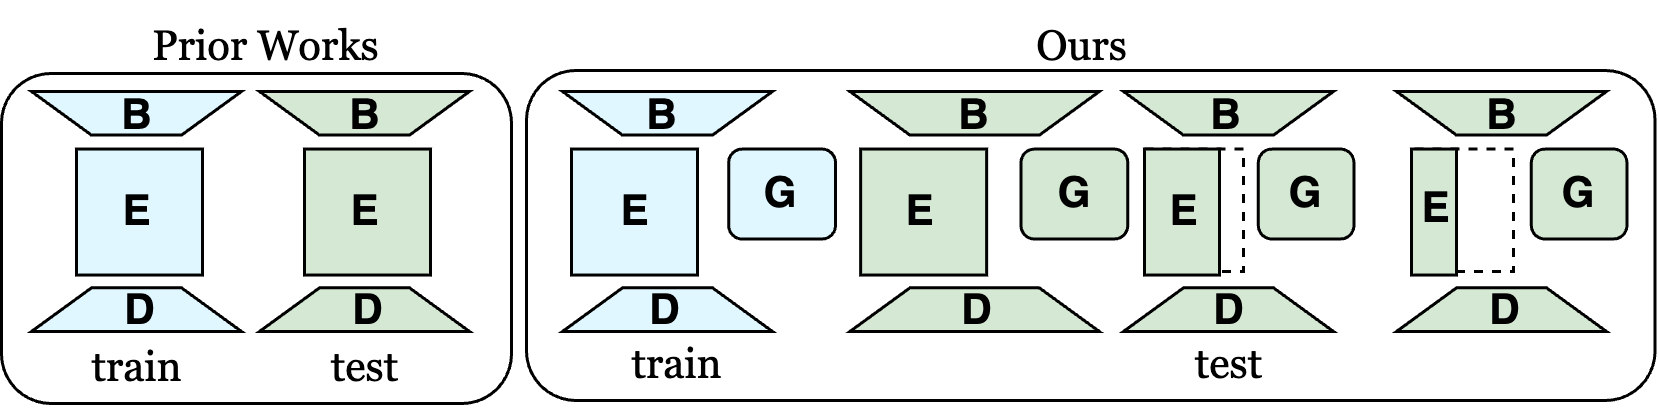
\includegraphics[width=\textwidth]{figures/images/teaser.png}
      \caption{\textbf{Comparison to prior works.} Instead of conventional M2F-style architecture that provides ``one-size-fits-all'' solution, our method \ours focuses on training such models in order to directly run at various resource encoder depths by leveraging a gating function. Here, \textbf{B}, \textbf{E}, \textbf{D}, and \textbf{G} denote the backbone, encoder, decoder, and (our proposed) gating network, respectively.} %
      \label{fig:teaser_a}
    \end{minipage}%
    \hfill
    \begin{minipage}{0.3\textwidth}
        \centering
        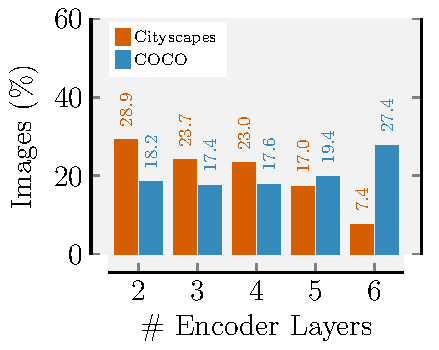
\includegraphics[width=\textwidth]{figures/images/image_vs_layer_barplot.pdf}
        \caption{Histogram of images achieving best panoptic segmentation by number of encoder layers.}
        \label{fig:teaser_b}
    \end{minipage}
    
\end{figure}